\documentclass[12pt,a4paper,leqno]{report}
\usepackage[utf8]{inputenc}
\usepackage[norsk]{babel}
\usepackage{amsmath}
\usepackage{amsfonts}
\usepackage{amssymb}
\usepackage{graphicx}
\usepackage{float}
\usepackage{tikz}

\usepackage[left=2cm,right=2cm,top=2cm,bottom=2cm]{geometry}
\author{Krister Borge}
\title{Labrapport \\ \small{prelab}}

\begin{document}
\maketitle
\textbf{Oppgave 1}

Spenningen over en oppladet kondensator med C=1 $\mu$ F
som er koblet til inngangen på et voltmeter halveres på 20 sekunder. Hva er indre resistansen til voltmeteret?\\
Kondensatoren og voltmeteret skaper denne kretsen:
\begin{figure}[H]
\caption{RC-krets}
\centering
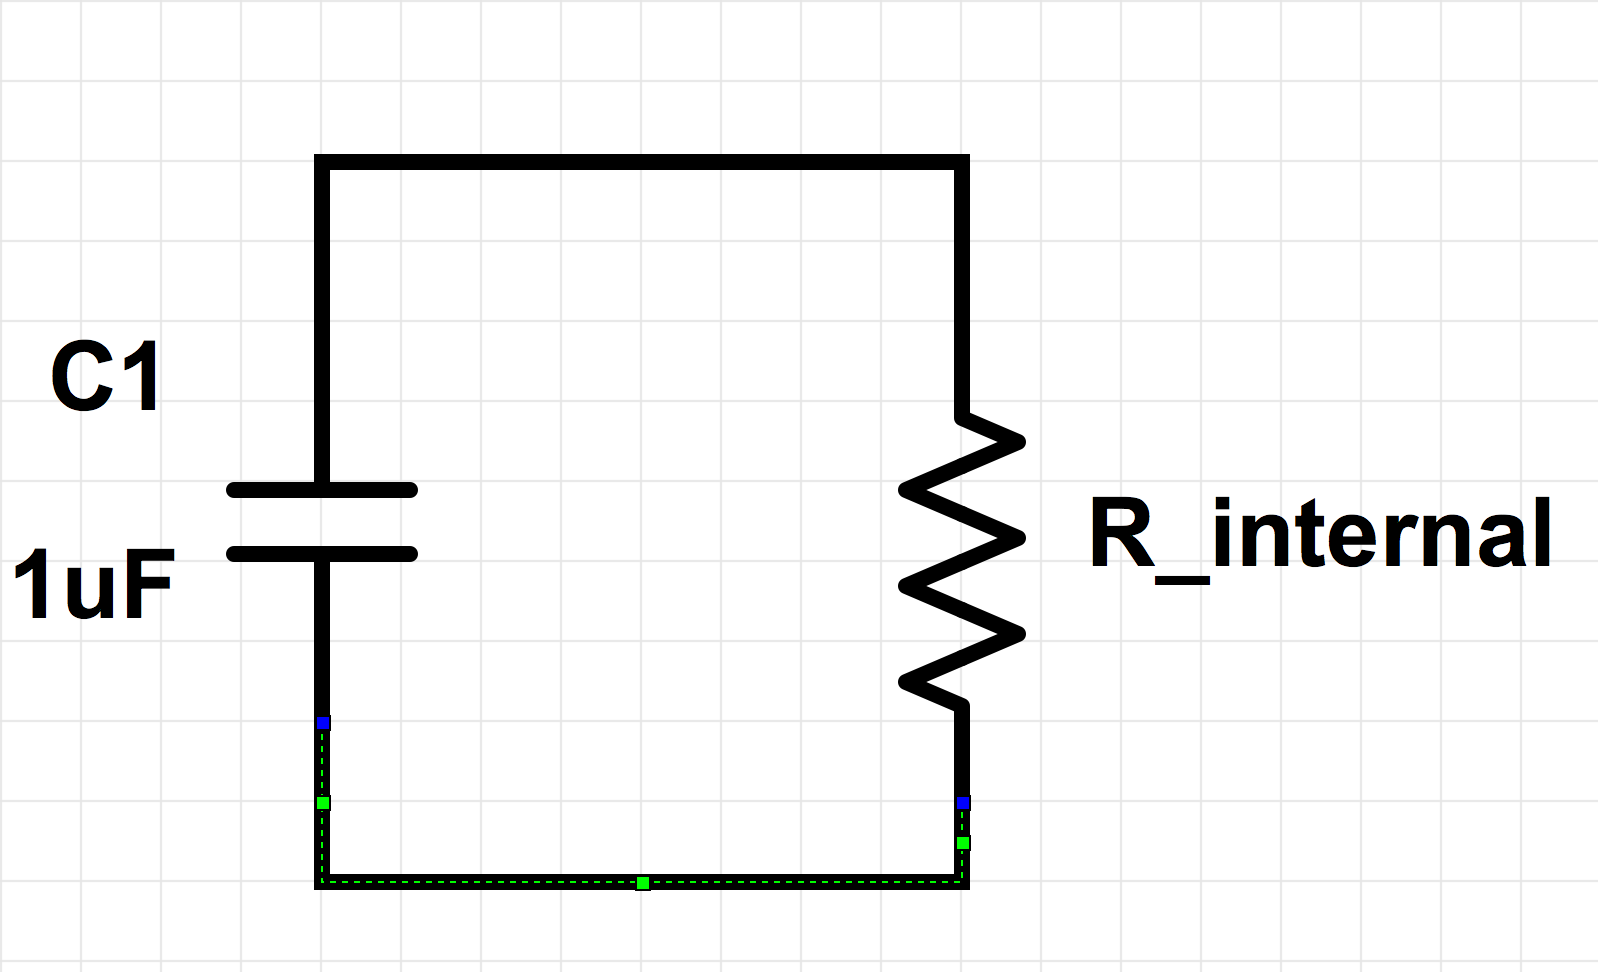
\includegraphics[width=\textwidth]{RC-cirquit.jpg}
\end{figure}
Jeg veit at $\tau=$RC. jeg veit også halveringstiden til kondensatoren som er 20 sekunder. Etter  1 $\tau$  er kondensatoren på 37\% av maks spenning. etter $t=20$ sekunder er spenningen lik $\frac{V_{max}}{2}$.
\begin{equation}
V(t)=V_0e^{-t/R_{internal}C}
\end{equation}

For RC-kretser gjelder:
\begin{equation}
\tau=RC
\end{equation}
men jeg har kondensator verdien og løser for R:
\begin{equation}
\ln(2)=\frac{t}{RC}
\end{equation}
\begin{equation}
\ln(2)=\frac{20}{RC}
\end{equation}
\begin{equation}
\ln(2)=\frac{20}{R1 \mu F}
\end{equation}
\begin{equation}
\ln(2)R=\frac{\frac{20}{10^{-6} F}}{\ln{2}}=\frac{20000000}{\ln(2)}=28853900,816=28,853900816\mathsf{M}\Omega
\end{equation}

Der $V_0$ er den initielle spenningen i kondensatoren.
Jeg har også at $Q_{max}=CV_{max}$
$F=\frac{Q}{V}$ 
\pagebreak
\textbf{Oppgave 2:} 

Lag et MATLAB-skript basert på metodene polyfit og polyval som tilpasser en linje til et sett med datapunkter x,y og viser punktene og den tilpassede linjen på en figur. Dette skriptet kan også brukes i labøvelse 3(Hall-effekt).

\begin{figure}
\caption{Matlabskript}
\begin{verbatim}
function []=lab1oppgave2(min, max, datapunkt,degree)
x = linspace(min,max,length(datapunkt));
y=datapunkt;
%
p = polyfit(x, datapunkt,degree);

x1 = linspace(min,max);
y1 = polyval(p,x1);
%plot
figure
plot(x,y,'or',x1,y1,'b')
title('Values and fitted curve')
legend('recorded values', 'fitted curve')

end
\end{verbatim}
\end{figure}
Dette kallet: 
\begin{verbatim}
>> lab1oppgave2(0,9,[1,2,5,7,16,19,11,15,11,19,11,15,14,19,11,15,13],7)
\end{verbatim}
gir dette plottet:
\begin{figure}[H]
\caption{Test av matlabskript}
\centering
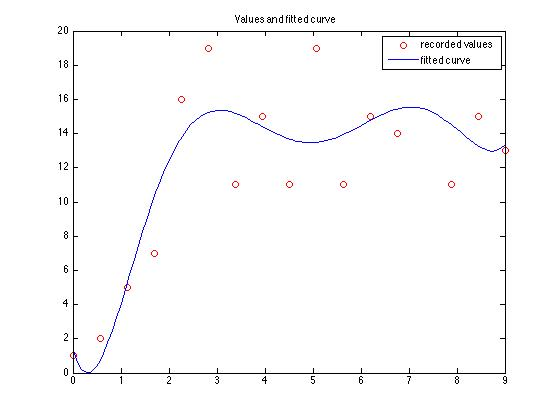
\includegraphics[width=\textwidth]{curvefittertest.jpg}
\end{figure}

\textbf{Oppgave 3:} 

Finn et uttrykk for $\mathbf{B}$ dersom vi dreier spolen med konstant vinkelhastighet $\omega$ og måler den maksimale verdien $\epsilon_0$ for $\epsilon(t)$. Hva er forholdet mellom 
$\omega$ og $t_0-t_1$?

Der spolens $N$ er spolens vindingstall og $A$ er spolens areal.
orientasjonen er slik at $\Phi(t_1)=NAB$ og 
\begin{equation}
2NAB=\int_{t1}^{t2}\epsilon(t)dt
\end{equation}
Jeg kan så se på hver del for seg:
\begin{equation}
\Phi(t_1)=2NAB\omega(t_1)=2NABcos(0)=2NB\pi r^2
\end{equation}
utrykt ved $B$ er dette:
\begin{equation}
B=\frac{\Phi(t_1)}{2N \pi r^2}
\end{equation}
\begin{equation}
\Phi(t_2)=2NAB\omega(t_2)=2NABcos(180)=-2NB\pi r^2
\end{equation}
utrykt ved $B$ er dette:
\begin{equation}
B=-\frac{\Phi(t_1)}{2N \pi r^2}
\end{equation}
Et utrykk for B kan da være:
\begin{equation}
B=\frac{\Phi(t_1)}{2N \pi r^2}-\frac{\Phi(t_1)}{2N \pi r^2}=\frac{\Phi(t_2)-\Phi(t_1)}{2N \pi r^2}
\end{equation}
Der $\Phi(T)$ kan utrykkes ved
\begin{equation}
-\int_{t1}^{t2}\epsilon(t)dt
\end{equation}

Amperes lov sier:
\begin{equation}
\oint \mathbf{B} ds=\mu_0I
\end{equation}
$\mu_0$ er permitiviteten.

Forholdet $\omega/t_1-t_2$:
\begin{equation}
\omega=\frac{2 \pi} {T}
\end{equation}


$t_2-t_1$ er området frem til $\cos(\pi)$:\\
Jeg skjønner det ikke!.	
\end{document}